%%%%%%%%%%%%%%%%%%%%%%%%%%%%%%%%%%%%%%%%%%%%%%%%%%%%%%%%%%%%%%%%%%%%%%%%%%%%%%%
\section{Results}
\label{sec:results}
%%%%%%%%%%%%%%%%%%%%%%%%%%%%%%%%%%%%%%%%%%%%%%%%%%%%%%%%%%%%%%%%%%%%%%%%%%%%%%%


%%%%%%%%%%%%%%%%%%%%%%%%%%%%%%%%%%%%%%%%%%%%%%%%%%%%%%%%%%%%%%%%%%%%%%%%%%%%%%%
\subsection{Eigenvalues}
\label{subsec:eigenvalues}

In the results that follow, the bias $\Delta\rho$ compares the eigenvalue $k_{eff}^{MOC}$ computed by OpenMOC to that of the reference eigenvalue $k_{eff}^{MC}$ computed by OpenMC in units of pcm:

\begin{equation}
\label{eqn:delta-rho}
\Delta\rho = \left(k_{eff}^{MOC} - k_{eff}^{MC}\right) \times 10^{5}
\end{equation}

\begin{table}[h!]
  \centering
  \caption{OpenMOC eigenvalue bias $\Delta\rho$.}
  \label{tab:keff-bias} 
  \begin{tabular}{l c c}
  \toprule
  \textbf{Benchmark} & \textbf{Null} & \textbf{Degenerate} \\
  \midrule
  Assembly & -161 & -161 \\
  Colorset & -142 & -132 \\
  \bottomrule
\end{tabular}
\end{table}


%%%%%%%%%%%%%%%%%%%%%%%%%%%%%%%%%%%%%%%%%%%%%%%%%%%%%%%%%%%%%%%%%%%%%%%%%%%%%%%
\subsection{Fission Rates}
\label{subsec:fiss-rates}

-add figures of spatial distribution of errors
-can I reproduce these plots? Do I have the batchwise.h5 results stored on my external hard drive??? If so, I should customize them for only 70 groups

\begin{table}[h!]
  \centering
  \caption{OpenMOC fission rate percent relative errors.}
  \label{tab:fiss-errors}
  \begin{tabular}{l l r r}
  \toprule
  \textbf{Benchmark} & \textbf{Metric} & \textbf{Null} & \textbf{Degenerate} \\
  \midrule
  \multirow{2}{*}{Assembly} & Max  & 0.380 & 0.315 \\
                            & Mean & 0.074 & 0.079 \\
  \midrule
  \multirow{2}{*}{Colorset} & Max  & 0.764 & 0.602 \\
                            & Mean & 0.178 & 0.138 \\
  \bottomrule
\end{tabular}
\end{table}

\begin{figure}[h!]
\centering
\begin{subfigure}{0.35\textwidth}
  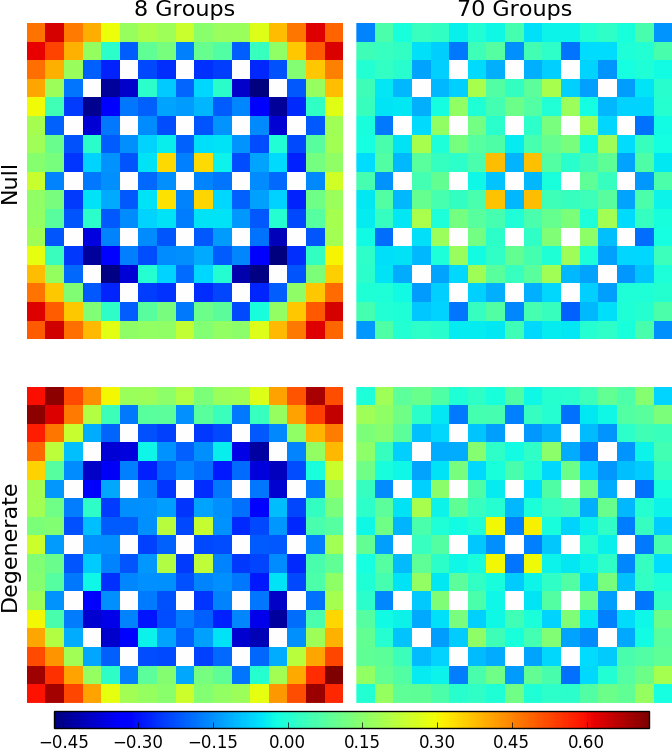
\includegraphics[width=\linewidth]{figures/assembly/fission-errors}
  \caption{}
  \label{fig:assm-fiss-error}
\end{subfigure}
\begin{subfigure}{0.35\textwidth}
  \centering
  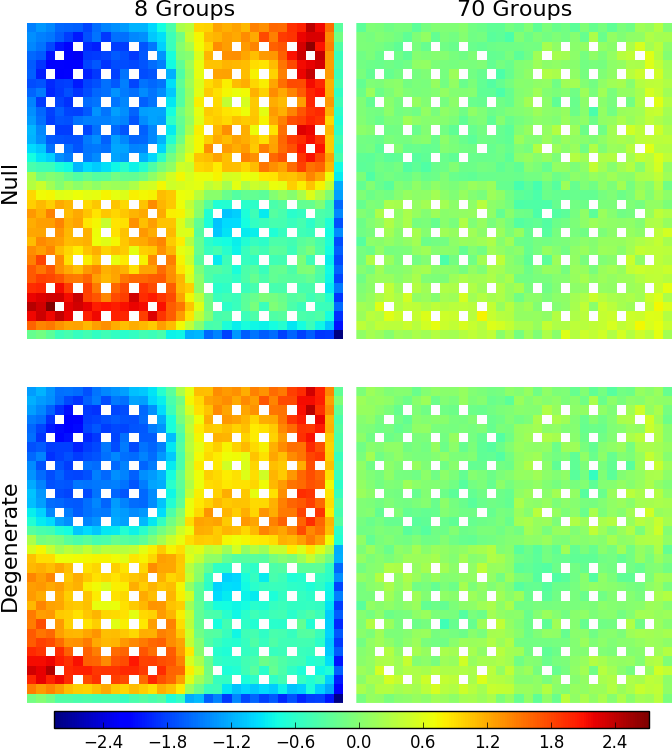
\includegraphics[width=\linewidth]{figures/reflector/fission-errors}
  \caption{}
  \label{fig:reflector-fiss-error}
\end{subfigure}
\caption{OpenMOC fission rate percent relative errors for the (a) assembly and (b) 2$\times$2 colorset models.}
\label{fig:fiss-errors}
\end{figure}


%%%%%%%%%%%%%%%%%%%%%%%%%%%%%%%%%%%%%%%%%%%%%%%%%%%%%%%%%%%%%%%%%%%%%%%%%%%%%%%
\subsection{Capture Rates}
\label{subsec:capt-rates}

-add figures of spatial distribution of errors

\begin{table}[h!]
  \centering
  \caption{OpenMOC U-238 capture rate percent relative errors.}
  \label{tab:capt-bias} 
  \begin{tabular}{l l r r}
  \toprule
  \textbf{Benchmark} & \textbf{Metric} & \textbf{Null} & \textbf{Degenerate} \\
  \midrule
  \multirow{2}{*}{Assembly} & Max  & -1.101 &  0.386 \\
                            & Mean &  0.479 &  0.086 \\
  \midrule
  \multirow{2}{*}{Colorset} & Max  & -1.969 & -0.783 \\
                            & Mean &  0.478 &  0.165 \\
  \bottomrule
\end{tabular}
\end{table}

\begin{figure}[h!]
\centering
\begin{subfigure}{0.35\textwidth}
  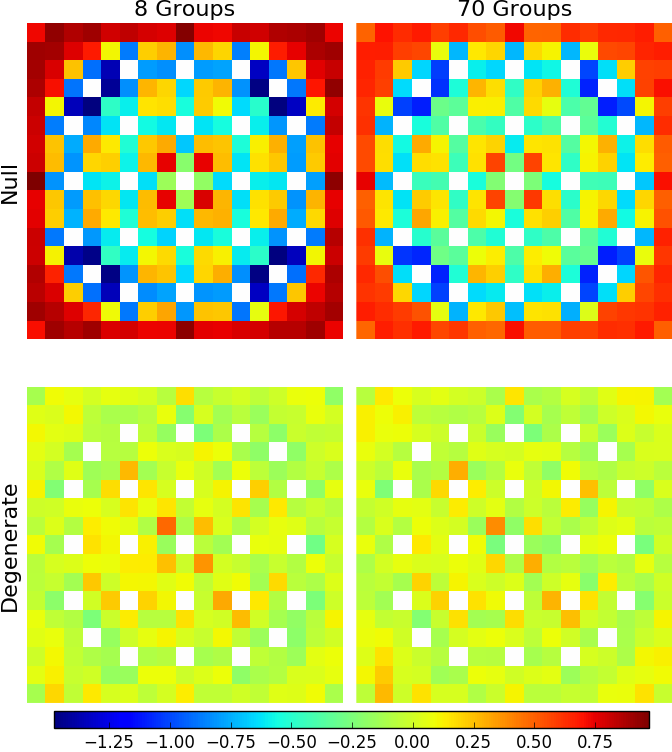
\includegraphics[width=\linewidth]{figures/assembly/capture-errors}
  \caption{}
  \label{fig:assm-capt-error}
\end{subfigure}
\begin{subfigure}{0.35\textwidth}
  \centering
  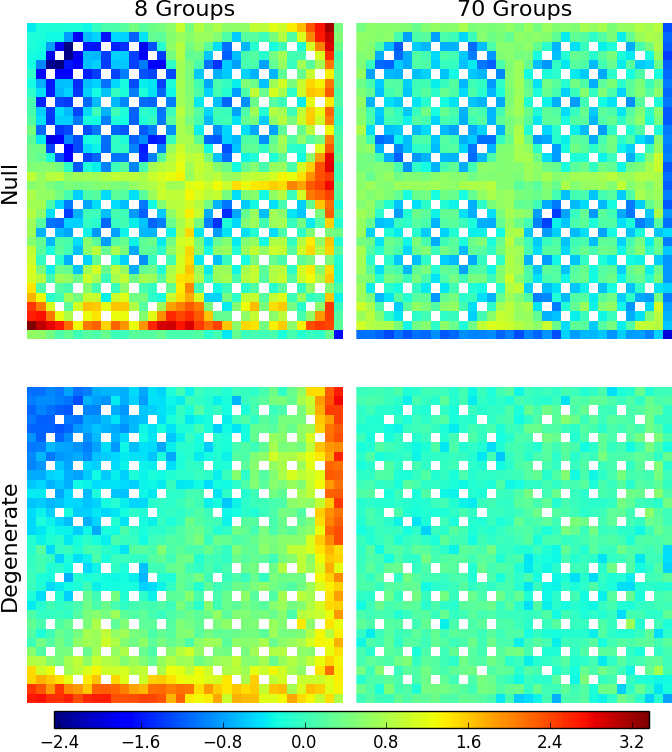
\includegraphics[width=\linewidth]{figures/reflector/capture-errors}
  \caption{}
  \label{fig:reflector-capt-error}
\end{subfigure}
\caption{OpenMOC U-238 capture rate percent relative errors for the (a) assembly and (b) 2$\times$2 colorset models.}
\label{fig:capt-errors}
\end{figure}

